
\section{PyPV: An easy Current-Voltage curves acquisition interface}

\epigraph{\textit{"Ok, I finally completed it, by the way, why did you start developing this?"\\"Well, it was just a proof of concept, but it's nice you worked on it"}}


	\subsection{Previous software}
		\begin{SCfigure}%[!hbtp]%
			\centering
			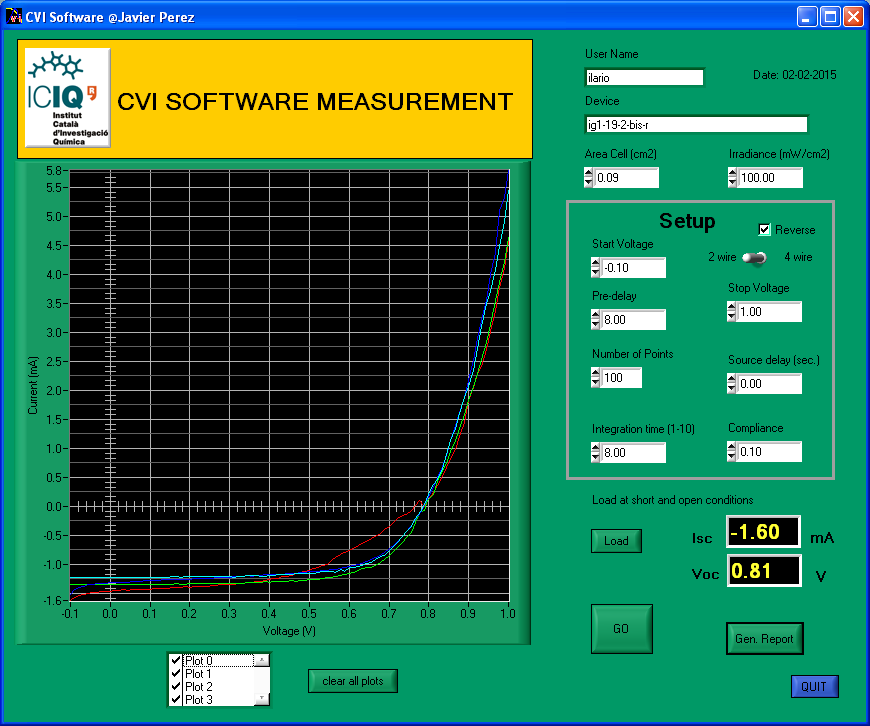
\includegraphics[width=0.5\textwidth]{old_iv_software/old_iv_software.png}
			\caption{}\label{fig:old_iv_software}
		\end{SCfigure}

	\subsection{Original Project}
		I received a proof-of-concept software developed by Daniel Fernandez Pinto and decided to continue the development. At that point the software had an interface with few buttons and a working Keithley communication library.

	\subsection{User's requests}
	\subsection{Implementation and user interface}

		\myparagraph{Autoscale} As it was explained in page~\pageref{autoscale}, the automatic scale setting of the Keithley is detrimental for perovskite solar cells dynamic measurements.

		\myparagraph{Auto-measure}\label{automeasure}
		
	\subsection{Limitations}
		
		The interface development has been started with the "Monkey Studio" software, which development has ceased even before the start of PyPV. This demonstrated to be a big failure in long term development planning.

\section{Robust and quick data analysis via R scripts}
\epigraph{\textit{"Is there an Origin version for Linux?"\\"No"}}


	\subsection{Charge Extraction (\acr{ce})}\label{r_ce}


	\subsection{Transient PhotoVoltage (\acr{tpv})}\label{r_tpv}
	
		\subsection{Transient PhotoCurrent (\acr{tpc})}\label{r_tpc}
		
			\subsection{Differential Capacitance (\acr{dc})}\label{r_dc}

\section{Maximum Power Point Tracking}\label{software_mppt}
\epigraph{\textit{"A student of mine sells a complete system for that, just buy it"}}

CITE Cimaroli2017

http://candlelight-systems.com/

\section{Time Resolved 1-D Drift and Diffusion Modelling}
	\subsection{Improvements and Additions to the DrIFtFUSION Core}
	\subsection{Impedance Spectroscopy}
	\subsection{ElectroAbsorption}
	
	\subsection{Ideality Factor}\label{dd_ideality}
		\myparagraph{Ideality Factor from \gls{voc}}
		
		\myparagraph{Ideality Factor from Current-Voltage Points}\label{dd_ideality_dark_jv}
https://www.pveducation.org/pvcdrom/characterisation/measurement-of-ideality-factor

\subsection{Techniques Which Could Be Implemented}
\epigraph{\textit{"Wow, this is a gold mine!"}}

\myparagraph{IMVS}

\myparagraph{IMPS}

\myparagraph{Mott-Schottky}
\url{https://en.wikipedia.org/wiki/Mott-Schottky_plot}